
\chapter{Phase Diversity Experiment} 
\label{ch:PDExp}

In this chapter, we will describe the experiment put in place in the optical laboratory at the HEIG-VD to reconstruct wavefronts with unknown static aberrations introduced using phase screens. At first, we study the  behavior of the phase diversity algorithm put in place by \citet{mugnier_2006} at ONERA with respect to number of averaging images, in other words noise level, and number of Zernike coefficients retrieved. Then we test the algorithm using a known aberration introduced by a parallel plane plate in the beam comparing the result to Zemax simulation. And finally, we introduce the phase screen to have random aberrations in the pupil and try to compare the phase diversity results with the Shack Hartman wavefront sensor results.

%------------------------------------------------------------------------------
%----------------------------------------------------------------------------

\section{ONERA algorithm}
\label{sec:ONERAalgorithm}



%----------------------------------------------------------------------------------------
%----------------------------------------------------------------------------------------

\section{Experimental Setup}
\label{sec:ExpSetup}

\begin{wrapfigure}{r}{0.5\textwidth}
\centering
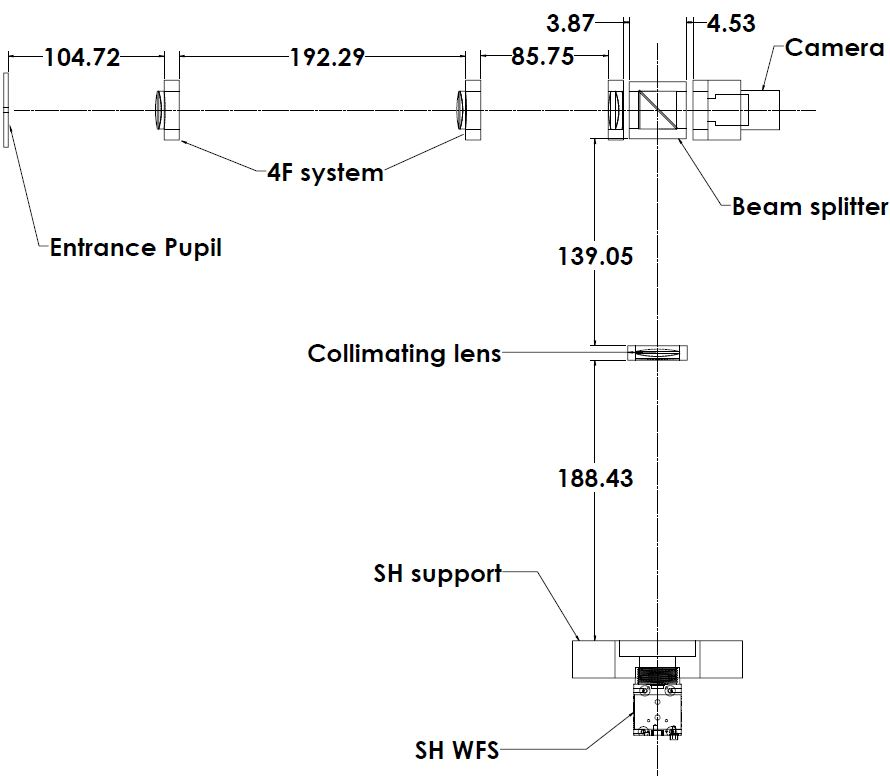
\includegraphics[width=0.5\textwidth]{Figures/setupSchema.JPG}
\decoRulewrapFig
\caption[Schema of the experimental setup]{Experimental setup schema with the relevant distances, \citep{Bouxin_PDM}.}
\label{fig:setupSchema}
\end{wrapfigure}

The design of the experiment was already done by \citet{Bouxin_PDM}. The system is built according to her plans and specifications.

The experiment is mounted on a pressurized legs optical table. The assembly contains six main components : a light source, an entrance pupil, an imaging system, a converging lens to focus the beam on the camera, a camera and a wavefront sensor.


\begin{table}
\caption[Optical Components]{Optical Components}
\label{tab:optComp}
\centering
\begin{tabular}{|l|l|l|c|}
\hline
\textbf{\#}& \textbf{Components} & \textbf{Model} & \textbf{Reference} \\\hline
1 & Pigtailed laser diode & Thorlabs, LPS-635-FC & \ref{app:pigtailedLaserDiode} \\\hline
2 & Converging lens, f = 11 mm & Thorlabs, A220TM-A & \ref{app:CL11} \\\hline
3 & Pinhole, 10 $\mu$m & Thorlabs, P10S & \ref{app:pinhole10microns} \\\hline
4 & Converging lens, f = 200 mm & Thorlabs, AL100200 & \ref{app:CL200} \\\hline
5 & 3.2 mm Hole milled in metal sheet & ... & ... \\\hline
6 & Converging lens, f = 100 mm & Thorlabs, AC254-100-A & \ref{app:CL100} \\\hline
7 & Converging lens, f = 80 mm & & \\\hline
8 & Camera CMOS & Ximea, MQ013MG-E2 & \ref{app:ximeaCam} \\\hline
9 & Converging lens, f = 100 mm & & \\\hline
10 & Shack-Hartman WFS & Thorlabs, WFS150-5C & \ref{app:SHwfs} \\\hline
\end{tabular}
\end{table}

\subsection{Light source}
\label{subsec:LigthSource}

\begin{wrapfigure}{r}{0.4\textwidth}
\centering
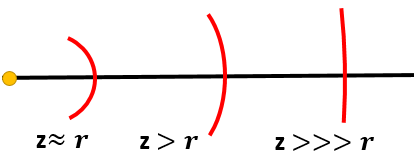
\includegraphics[width=0.4\textwidth]{Figures/WFdistantSource.PNG}
\decoRulewrapFig
\caption[Wavefront curvature]{Wavefront curvature for different point source's distances, \textit{z}. \textit{r} represents the characteristic size of the arc of interest.}
\label{fig:WFdistantSource}
\end{wrapfigure}

The final application of the phase diversity will be to characterize the optical aberrations induced by the imperfect optical path to a scientific detector of a telescope. For this reason, the light source has to simulate a distant star aberration-free wavefront. A distant star wavefront is considered planar since the object distance, z, is far greater than the telescope size, r, see Fig. \ref{fig:WFdistantSource}. The source of our experiment must then be characterized by a planar wavefront.

In order to obtain such a planar wavefront at the entrance pupil, the light source consist of a "pigtailed laser diode", a f=11mm converging lens, a pinhole and a f=200 mm converging lens, see Table \ref{tab:optComp}. The pigtailed laser diode emits a Gaussian beam centred at 637.5 nm slightly diverging. The converging lens concentrates the beam at the center of the 10$\mu$m pinhole to filter the noise. The second converging lens collimates the beam, obtaining a collimated beam with a planar wavefront, see Fig. \ref{fig:sourceRayTracing} and \ref{fig:pinholeEffect}.

\begin{figure}
\centering
    \begin{subfigure}{0.5\textwidth}
        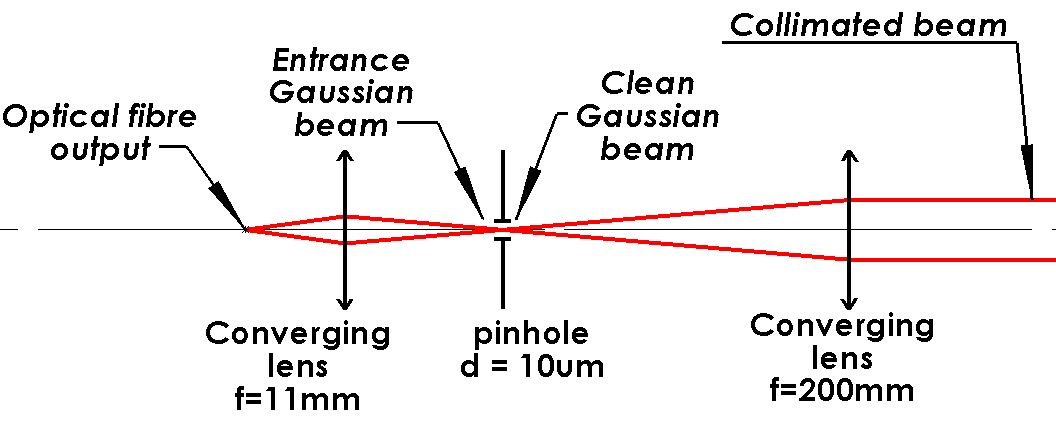
\includegraphics[width=\textwidth]{Figures/source.png}
        \caption{Source ray tracing.}
        \label{fig:sourceRayTracing}
    \end{subfigure}
    \quad
    \begin{subfigure}{0.3\textwidth}
        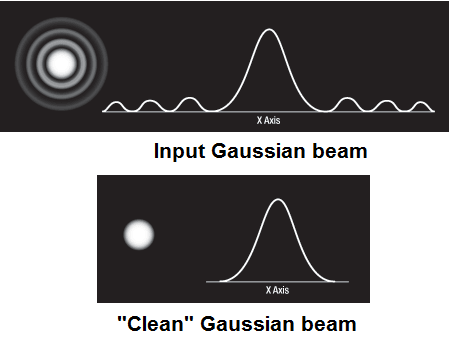
\includegraphics[width=\textwidth]{Figures/pinholeEffect.png}
        \caption{Beam view before and after the pinhole, \citep{SpatialFilters}.}
        \label{fig:pinholeEffect}
    \end{subfigure}
    \decoRule
    \caption{Source schema and pinhole effect on the beam.}
\end{figure}

\subsection{Entrance pupil}
\label{subsec:EntrancePupil}

The entrance pupil of our optical system is a circular aperture of 3.2 mm diameter placed after the collimating lens of the light source. It is milled in a metal plate and centred in his support, to avoid positioning with a XY table. The diameter is chosen in available material to fit in the different detector's surfaces.

\subsection{Pupil imaging system}
\label{subsec:pupilImSystem}

The phase diversity technique requires PSFs images as input, which means that the beam as to be focused onto the detector surface. To analyse the aberration in the pupil plane, one needs to focus an image of the beam passing through the entrance pupil. The simplest assembly to achieve this goal is the 4F system, which consist of two converging lenses of focal 100 mm. The two lenses are separated by 200 mm, see Fig. \ref{fig:setupSchema}. This places the image of the entrance pupil 100 mm after the second converging lens.

\subsection{Detectors}
\label{subsec:Detectors}

The image of the entrance pupil, obtained with the 4F system, is focused onto a CMOS Ximea camera by a f = 80 mm converging lens to acquire the PSFs for the phase diversity wavefront retrieval. The camera has a surface composed by 1280x1024 pixels of 5.3 $\mu$m, see Appendix \ref{app:ximeaCam}. It is mounted on sliding support in order to be able to acquire in/out-of-focus images. A beam splitter is placed in the converging beam to separate it in two. The second beam is collimated and a Shack-Hartman WFS is placed on the entrance pupil image plane, to check the results of the phase diversity wavefront retrieval. The Shack-Hartman WFS has a 39 X 31 lenslets grid and a CCD with a resolution of 1280x1024 pixels of 4.65 $\mu$m, see Appendix \ref{app:SHwfs}. 

%------------------------------------------------------------------------------
%	SECTION 2
%----------------------------------------------------------------------------

\section{Data Acquisition}
\label{sec:DataAcquis}

\subsection{Ximea Camera}
\label{subsec:acquisXimCam}

The ONERA algorithm takes one focused and one defocused PSFs, as said in section \ref{sec:ONERAalgorithm}. The PSFs are acquired using a python script which uses an open-source library to control the ximea camera, \verb|pyXimea|\footnote{\url{https://github.com/pupil-labs/pyximea}}, available on GitHub. The acquisition is done following these steps : 

\begin{enumerate}

\item The first step in order to acquire PSFs is to determine the position of the camera's focus point using the python script \verb|AlignementScriptXimeaCamera.py|, see Appendix \ref{app:AlignementScriptXimeaCamera}. This script let's you acquire consecutively PSFs at different camera's positions and computes their FWHM. It finally returns the minimum FWHM and the camera's position, see Figure \ref{fig:28092017AlignementXimeaPSFs}.

\begin{center}
\begin{figure}
\includegraphics[width=\textwidth]{../../../fig/alignement/28092017AlignementXimeaPSFs.png}
\caption{PSFs example of an alignment procedure}
\label{fig:28092017AlignementXimeaPSFs}
\end{figure}
\end{center}

\item Once you have the focus point position 

\end{enumerate}

\subsection{Shack-Hartman WFS}
\label{subsec:acquisSHwfs}

%------------------------------------------------------------------------------
%----------------------------------------------------------------------------

\section{Results}
\label{sec:Results}

This section presents the results of the phase diversity experiment, with the introduction of different sources of aberration.

\subsection{Parallel plane plate}
\label{subsec:ParPlanePlate}

The first source of aberration studied in this work is a tilted parallel plane plate which is used as a calibrated source of astigmatism.
